\documentclass{article}
\usepackage{fancyhdr}
\usepackage[table]{xcolor}
\usepackage[margin=1in]{geometry}
\usepackage{caption}
\usepackage{hyperref}
\usepackage{graphicx}
\usepackage{float}
\usepackage{enumitem}
\usepackage{array}
\usepackage{tikz}
\usetikzlibrary{shapes.geometric, arrows, fit}

% Define TikZ styles
\tikzstyle{startstop} = [rectangle, rounded corners, minimum width=3cm, minimum height=1cm, text centered, draw=black, fill=red!30]
\tikzstyle{process} = [rectangle, minimum width=3cm, minimum height=1cm, text centered, draw=black, fill=blue!10]
\tikzstyle{arrow} = [thick,->,>=stealth]
\tikzstyle{input} = [rectangle, draw, fill=white, minimum height=1cm, minimum width=2cm, text centered]


% Set header and footer
\pagestyle{fancy}
\fancyhf{}
\fancyhead[L]{USC Facilities: Rain Barrel Water Pump System[Handout 3]} % Team name in the header
\fancyfoot[C]{\thepage} % Page number in the footer

\begin{document}

\thispagestyle{fancy} % Ensures header and footer are applied to cover page

\newpage

\section*{Functional Diagram}

\begin{figure}[htbp]
    \centering
\resizebox{\textwidth}{!}{%
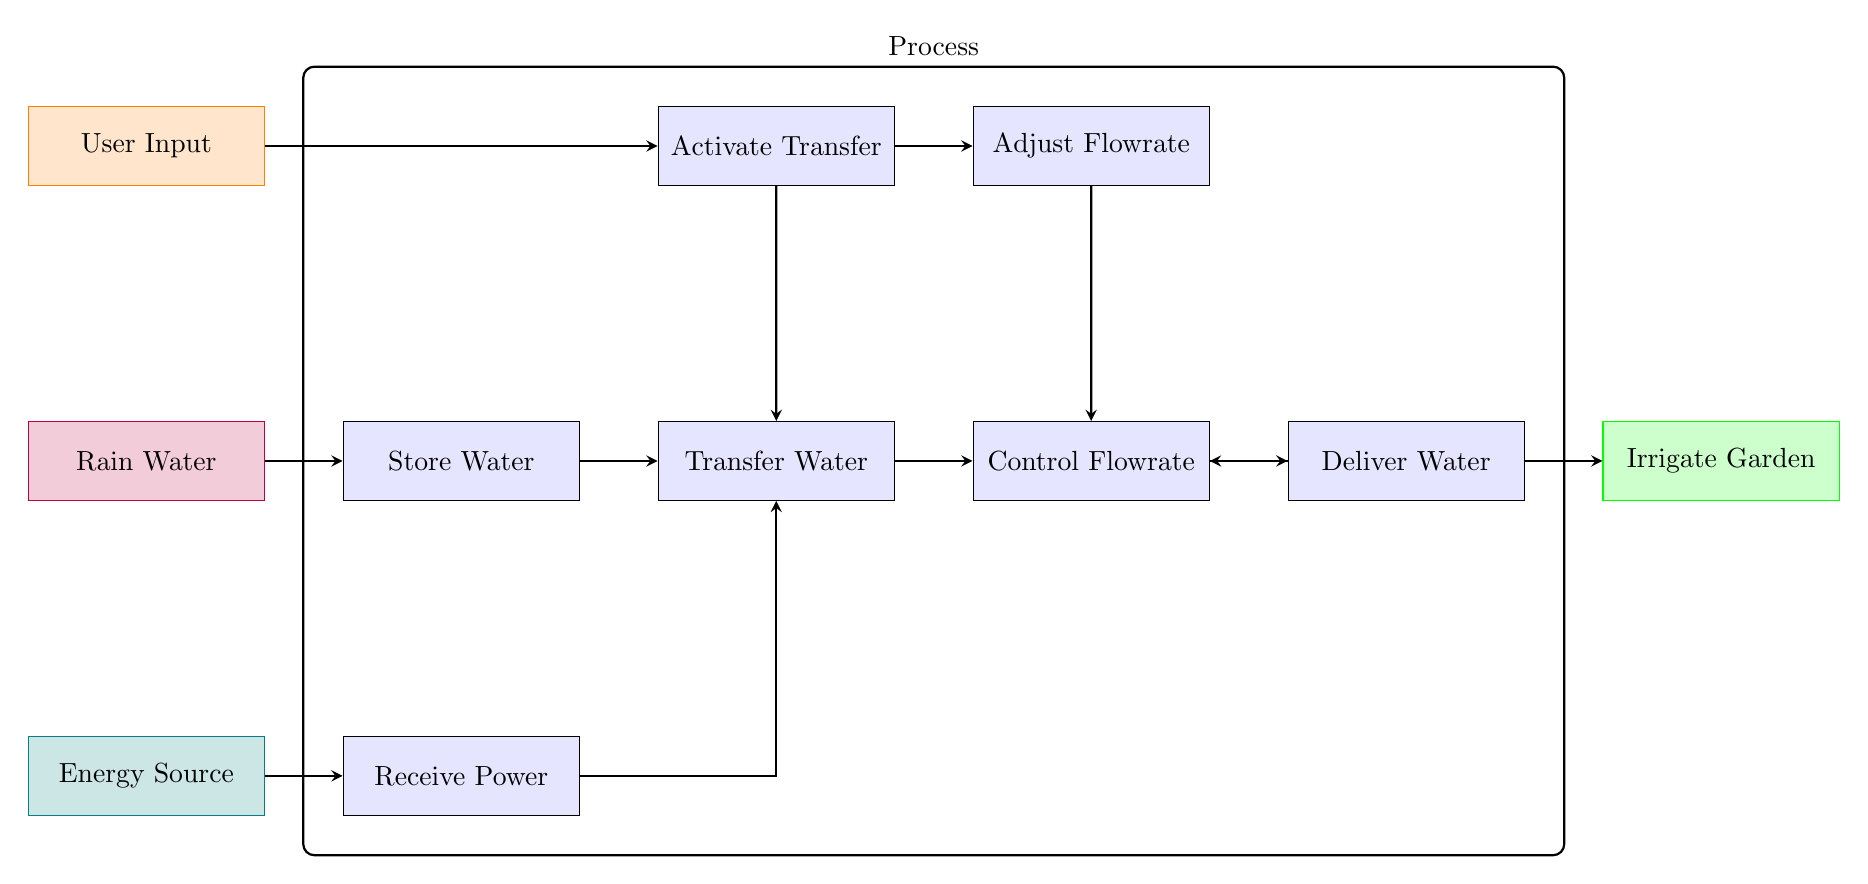
\begin{tikzpicture}[node distance=2cm]

% Input Nodes
\node (userinput) [input, draw=orange, fill=orange!20, minimum width=3cm, minimum height=1cm] {User Input};
\node (rainwater) [input, below of=userinput, yshift=-2cm, draw=purple, fill=purple!20, minimum width=3cm, minimum height=1cm] {Rain Water};
\node (energysource) [input, below of=rainwater, yshift=-2cm, draw=teal, fill=teal!20, minimum width=3cm, minimum height=1cm] {Energy Source};


% Process Nodes
\node (activatetransfer) [process, right of=userinput, xshift=6cm] {Activate Transfer};
\node (storewater) [process, right of=rainwater, xshift=2cm] {Store Water};
\node (receivepower) [process, right of=energysource, xshift=2cm] {Receive Power};
\node (adjustflowrate) [process, right of=activatetransfer, xshift=2cm] {Adjust Flowrate};
\node (transferwater) [process, right of=storewater, xshift=2cm] {Transfer Water};
\node (controlflowrate) [process, right of=transferwater, xshift=2cm] {Control Flowrate};
\node (deliverwater) [process, right of=controlflowrate, xshift=2cm] {Deliver Water};

% Output Node
\node (irrigategarden) [input, right of=deliverwater, xshift=2cm, draw=green, fill=green!20, minimum width=3cm, minimum height=1cm] {Irrigate Garden};
% Background Rectangle covering internal process
\node[draw=black, thick, rounded corners, fit=(activatetransfer)(storewater)(receivepower)(adjustflowrate)(transferwater)(controlflowrate)(deliverwater), inner sep=0.5cm, label={[above]Process}] {};

% Arrows between nodes
\draw [arrow] (userinput) -- (activatetransfer);
\draw [arrow] (activatetransfer) -- (adjustflowrate);
\draw [arrow] (rainwater) -- (storewater);

\draw [arrow] (storewater) -- (transferwater);
\draw [arrow] (transferwater) -- (controlflowrate);
\draw [arrow] (controlflowrate) -- (deliverwater);
\draw [arrow] (deliverwater) -- (irrigategarden);
\draw [arrow] (energysource) -- (receivepower);
\draw [arrow] (receivepower) -| (transferwater);
\draw [arrow] (activatetransfer) -- (transferwater);
\draw [arrow] (adjustflowrate) -- (controlflowrate);

\draw [arrow] (deliverwater) -- (controlflowrate);

\end{tikzpicture}
}  

    \caption{Functional Decomposition Diagram}

\end{figure}

\newpage

\section*{Concept Combination Tables}

\begin{table}[h!]
    \centering
    \caption{Concept Combination Table for the Efficient Water Transfer System}
    
\includegraphics[width=1\textwidth]{FD_Report/CCT.png} % Ensure the image file is correctly referenced
    \label{tab:concept_combination_table}
\end{table}
\newpage
\begin{table}[h!]
    \centering
    \caption{Shortened Concept Combination Table}
    
\includegraphics[width=1\textwidth]{FD_Report/CCT_selected.png}
\end{table}


\newpage

\section*{Current System Description}

\subsection*{Overview}

\begin{figure}[h!]
    \centering
    
\includegraphics[width=0.8\textwidth]{FD_Report/figure1.png} % Placeholder for Figure 1
    \caption{Current System for Water Transfer}
    \label{fig:current_system}
\end{figure}

The current system uses a 7-foot-tall tank to store water. However, it does not utilize the available height effectively to generate sufficient pressure. Although the tank can theoretically provide a pressure of 3.03 PSI, the actual flow rate measured is only 2.2 GPM through a standard ¾" garden hose. Significant pressure losses reduce the pressure to almost zero by the time the water reaches the garden. This inefficiency results in ineffective irrigation, as water does not flow efficiently from the tank to the garden.

\subsection*{Key Issues in the Current System}

\begin{itemize}
    \item \textbf{Limited Pressure}: Maximum achievable pressure is 4 PSI before losses, which is insufficient for effective flow.
    \item \textbf{Low Flow Rate}: Measured at only 2.2 GPM, resulting in slow water transfer.
    \item \textbf{Inefficient Water Flow}: Water struggles to reach the garden due to elevation differences and friction losses in the hose.
    \item \textbf{User Experience}: Slow flow means it takes 55 seconds to fill a 2-gallon can, which is inefficient for gardening needs.
\end{itemize}

\newpage

\section*{Concept 1: Modified System Using a 2-Inch Pipe}

\begin{figure}[h!]
    \centering
    
\includegraphics[width=0.8\textwidth]{FD_Report/figure2.png} % Placeholder for Figure 2
    \caption{Modified System Concept Using 2-Inch Pipe}
    \label{fig:modified_system}
\end{figure}

This concept aims to improve pressure and flow rate by replacing the garden hose with a wider 2-inch pipe, minimizing friction losses and better leveraging the tank’s existing pressure.

\subsection*{How the Concept Works}
\begin{itemize}
    \item \textbf{Larger Pipe Diameter}: The 2-inch pipe allows for greater flow, improving the transfer rate to over 20 GPM.
    \item \textbf{Pressure Utilization}: Maintains a flow pressure of approximately 4 PSI, even after losses.
    \item \textbf{Fast Water Transfer}: Allows a 2-gallon can to be filled in 6 seconds.
    \item \textbf{Cost and Simplicity}: Minimal in cost and complexity, requiring only the replacement of the garden hose with a larger pipe.
    \item \textbf{Limitations}: Cannot use garden hoses or sprinklers due to design changes; optimized for fast manual water transfers.
\end{itemize}

\subsection*{Addressing the Identified Functions}
\begin{enumerate}
    \item \textbf{Activation of Transfer}: Manually by opening the pipe valve.
    \item \textbf{Adjustment of Flowrate}: Controlled using a valve on the 2-inch pipe.
    \item \textbf{Storing Water}: The 7-foot tank continues to store water without changes.
    \item \textbf{Transferring Water}: Ensures rapid water transfer with minimal resistance.
    \item \textbf{Controlling Flowrate}: Achieved through manual valves on the pipe.
\end{enumerate}

\newpage

\section*{Concept 2: Gravity System by Raising the Tank}

\begin{figure}[h!]
    \centering
    
\includegraphics[width=0.5\textwidth]{FD_Report/figure3.png} % Placeholder for Figure 3
    \caption{Gravity System Concept}
    \label{fig:gravity_system}
\end{figure}

The gravity system increases water pressure and flow rate by elevating the 7-foot tank to a height where the combined height difference between the tank and garden becomes 14 feet, leveraging gravity to enhance natural pressure without electric pumps.

\subsection*{How the Concept Works}
\begin{itemize}
    \item \textbf{Increased Pressure through Elevation}: Elevating the tank increases the outlet pressure to around 10 PSI.
    \item \textbf{Improved Usability}: Makes the use of a standard ¾” garden hose more practical.
    \item \textbf{Simple Operation}: Water flows through a 2-inch pipe to minimize friction losses before transitioning to a garden hose.
    \item \textbf{Safety Concerns}: Requires secure support for the elevated tank, necessitating proper installation and regular inspection.
    \item \textbf{Potential Water Flow Rate}: Enhances water transfer speed, providing a faster fill time for a 2-gallon can.
\end{itemize}

\subsection*{Addressing the Identified Functions}
\begin{enumerate}
    \item \textbf{Activation of Transfer}: Opening a valve at the tank outlet.
    \item \textbf{Adjustment of Flowrate}: Manual valves on both the 2-inch pipe and the garden hose.
    \item \textbf{Storing Water}: Utilizes the existing 1000-gallon tank.
    \item \textbf{Transferring Water}: Rapid transfer through the 2-inch pipe with minimal friction losses.
    \item \textbf{Controlling Flowrate}: Dual-valve system for precise control.
    \item \textbf{Delivering Water}: Delivers water via the garden hose under increased pressure.
\end{enumerate}

\newpage

\section*{Concept 3: Manual Pump System}

\begin{figure}[h!]
    \centering
    
\includegraphics[width=0.65\textwidth]{FD_Report/figure4.png} % Placeholder for Figure 4
    \caption{Manual Pump System Concept}
    \label{fig:manual_pump}
\end{figure}

This concept introduces a manual pump apparatus to increase water pressure and flow, relying on human energy to operate a pump connected to the 2-inch pipe.

\subsection*{How the Concept Works}
\begin{itemize}
    \item \textbf{Manual Pumping}: Operated by a user to draw water from the 7-foot tank and push it through a 2-inch pipe.
    \item \textbf{Increased Control}: Provides flexibility between flow rate and pressure.
    \item \textbf{Labor Requirements}: Optimal operation may require two people.
    \item \textbf{Usage Complexity}: Adds operational complexity and cost due to the need for the pump apparatus.
    \item \textbf{Output Performance}: Depends on pump specifications, determining PSI or GPM achieved.
\end{itemize}

\subsection*{Addressing the Identified Functions}
\begin{enumerate}
    \item \textbf{Activation of Transfer}: Operating the manual pump.
    \item \textbf{Adjustment of Flowrate}: Controlling pump speed or effort.
    \item \textbf{Storing Water}: Utilizes the existing 7-foot, 1000-gallon tank.
    \item \textbf{Transferring Water}: Connects the 2-inch pipe to the pump apparatus to minimize resistance.
    \item \textbf{Controlling Flowrate}: Dynamic adjustment based on user input.
    \item \textbf{Delivering Water}: Directed to different garden areas as needed.
\end{enumerate}

\newpage \section*{Concept 4: Pump System with Raised Tank}

\begin{figure}[h!]
    \centering
    
\includegraphics[width=0.8\textwidth]{FD_Report/figure5.png} % Placeholder for Figure 5
    \caption{Pump System with Raised Tank}
    \label{fig:pump_raised_tank}
\end{figure}

This concept combines a raised secondary tank with a manual pump to increase pressure and flow rate, blending manual effort with gravity for efficient water delivery.

\subsubsection*{How the Concept Works}
\begin{itemize}
    \item \textbf{Pump to Raised Tank}: Manual pump transfers water from the main tank to the elevated secondary tank.
    \item \textbf{Increased Pressure from Elevation}: Height of the raised tank determines the pressure and improves water delivery.
    \item \textbf{Constant Pumping Required}: Pressure is maintained only if the raised tank is kept filled.
    \item \textbf{Flow and Pressure Control}: Influenced by the height of the secondary tank and pump specifications.
    \item \textbf{Complexity and Costs}: More complex and costly due to the additional tank and secure elevation requirements.
\end{itemize}

\subsubsection*{Addressing the Identified Functions}
\begin{enumerate}
    \item \textbf{Activation of Transfer}: Operating the manual pump.
    \item \textbf{Adjustment of Flowrate}: Valves on the raised tank and pipe system.
    \item \textbf{Storing Water}: Water stored in both the main and raised tanks.
    \item \textbf{Transferring Water}: From the primary tank to the raised tank via the pump.
    \item \textbf{Controlling Flowrate}: Valves on the raised tank’s outlet.
    \item \textbf{Delivering Water}: Under higher pressure from the raised tank to the garden.
\end{enumerate}

\newpage \section*{Concept 5: Pump System with Pressure Tank}

\begin{figure}[h!]
    \centering
    
\includegraphics[width=0.8\textwidth]{FD_Report/figure6.png} % Placeholder for Figure 6
    \caption{Pump System with Pressure Tank}
    \label{fig:pump_pressure_tank}
\end{figure}

Integrates a manual pump with a pressure tank to provide stable and controlled water flow, enhancing usability by balancing flow rate and pressure.

\subsubsection*{How the Concept Works}
\begin{itemize}
    \item \textbf{Pumping into a Pressure Tank}: Manual pump transfers water from the primary tank into the pressure tank.
    \item \textbf{Maintaining Pressure}: Pressure tank stores water under higher pressure based on tank design.
    \item \textbf{Stable Water Delivery}: Consistent flow without constant pumping.
    \item \textbf{Design Complexity}: Adds complexity and cost due to the specialized pressure tank.
    \item \textbf{Challenges}: Larger pressure tanks require more time and effort to fill and maintain proper pressure levels.
\end{itemize}

\subsubsection*{Addressing the Identified Functions}
\begin{enumerate}
    \item \textbf{Activation of Transfer}: Manual pumping into the pressure tank.
    \item \textbf{Adjustment of Flowrate}: Valve on the pressure tank's outlet.
    \item \textbf{Storing Water}: Stored in both the main and pressure tanks.
    \item \textbf{Transferring Water}: From the primary tank to the pressure tank via the pump.
    \item \textbf{Controlling Flowrate}: Stable flow control via the pressure tank.
    \item \textbf{Delivering Water}: Consistent pressure from the pressure tank.
\end{enumerate}

\newpage \section*{Concept 6: Solar Pump System}

\begin{figure}[h!]
    \centering
    
\includegraphics[width=0.6\textwidth]{FD_Report/figure7.png} % Placeholder for Figure 7
    \caption{Solar Pump System Concept}
    \label{fig:solar_pump}
\end{figure}

Introduces renewable energy by utilizing a solar-powered pump, reducing reliance on manual labor and external power sources while considering limitations related to flow rate and sunlight availability.

\subsubsection*{How the Concept Works}
\begin{itemize}
    \item \textbf{Solar-Powered Operation}: Solar panels power the pump to draw water from the primary tank.
    \item \textbf{Daylight Dependency}: Operates only during sufficient sunlight hours.
    \item \textbf{Limited Flow and Pressure}: Dependent on pump specifications and solar panel power.
    \item \textbf{Design Complexity}: Increased complexity and cost due to the addition of solar panels and pumps.
\end{itemize}

\subsubsection*{Addressing the Identified Functions}
\begin{enumerate}
    \item \textbf{Activation of Transfer}: Automatic activation by sunlight.
    \item \textbf{Adjustment of Flowrate}: Pump settings or outlet valve adjustments.
    \item \textbf{Storing Water}: Utilizes the main 1000-gallon tank.
    \item \textbf{Transferring Water}: Pumped through the 2-inch pipe to the garden.
    \item \textbf{Controlling Flowrate}: Influenced by solar pump performance.
    \item \textbf{Delivering Water}: Under pressure, though limited compared to electric pumps.
\end{enumerate}

\newpage \section*{Concept 7: Solar-Powered Pump with Raised Tank System}

\begin{figure}[h!]
    \centering
    
\includegraphics[width=0.8\textwidth]{FD_Report/figure9.png} % Placeholder for Figure 8
    \caption{Solar + Raised Tank System Concept}
    \label{fig:solar_raised_tank}
\end{figure}

Combines a solar-powered pump with a raised secondary tank to create a high-pressure water delivery system, leveraging both renewable energy and gravitational force.

\subsubsection*{How the Concept Works}
\begin{itemize}
    \item \textbf{Solar-Powered Pump to Raised Tank}: Transfers water from the main tank to an elevated secondary tank.
    \item \textbf{Improved Pressure and Flow}: Steady pressure determined by the height of the raised tank.
    \item \textbf{Operational Limitations}: Operates only during daylight hours.
    \item \textbf{Structural Challenges}: Requires stable structure to support the elevated tank.
    \item \textbf{System Complexity and Cost}: Increased complexity and cost due to solar panels and raised tank.
\end{itemize}

\subsubsection*{Addressing the Identified Functions}
\begin{enumerate}
    \item \textbf{Activation of Transfer}: Solar pump activated by sunlight.
    \item \textbf{Adjustment of Flowrate}: Valves at the raised tank outlet.
    \item \textbf{Storing Water}: Stored in both primary and raised tanks.
    \item \textbf{Transferring Water}: From the primary tank to the raised tank via the solar pump.
    \item \textbf{Controlling Flowrate}: Stable pressure control via the raised tank.
    \item \textbf{Delivering Water}: Under higher pressure from the raised tank.
\end{enumerate}

\newpage \section*{Concept 8: Solar-Powered Pump with Pressure Tank System}

\begin{figure}[h!]
    \centering
    
\includegraphics[width=0.8\textwidth]{FD_Report/figure8.png} % Placeholder for Figure 9
    \caption{Solar + Pressure Tank System Concept}
    \label{fig:solar_pressure_tank}
\end{figure}

Combines a solar-powered pump with a pressure tank to maintain steady water pressure and flow, ensuring more consistent performance despite intermittent sunlight.

\subsubsection*{How the Concept Works}
\begin{itemize}
    \item \textbf{Solar-Powered Pump to Pressure Tank}: Transfers water from the main tank to the pressure tank using solar energy.
    \item \textbf{Pressurized Water Delivery}: Stores water under pressure for consistent flow.
    \item \textbf{Flow and Pressure Control}: Determined by tank design and pump capabilities.
    \item \textbf{Intermittent Operation}: May experience interruptions during low sunlight.
    \item \textbf{System Complexity and Cost}: Increased due to the addition of solar panels and pressure tanks.
\end{itemize}

\subsubsection*{Addressing the Identified Functions}
\begin{enumerate}
    \item \textbf{Activation of Transfer}: Pump activated by sunlight.
    \item \textbf{Adjustment of Flowrate}: Valve on the pressure tank outlet.
    \item \textbf{Storing Water}: Stored in both main and pressure tanks.
    \item \textbf{Transferring Water}: From main tank to pressure tank via solar pump.
    \item \textbf{Controlling Flowrate}: Stable flow control via pressure tank.
    \item \textbf{Delivering Water}: Consistent pressure delivery from the pressure tank.
\end{enumerate}

\newpage \section*{Concept 9: Battery-Powered Pump System}

\begin{figure}[h!]
    \centering
    
\includegraphics[width=0.8\textwidth]{FD_Report/figure10.png} % Placeholder for Figure 10
    \caption{Battery Pump System Concept}
    \label{fig:battery_pump}
\end{figure}

Introduces a battery-powered pump to draw water from the primary tank, offering more consistent performance compared to solar systems but requiring regular battery maintenance.

\subsubsection*{How the Concept Works}
\begin{itemize}
    \item \textbf{Battery-Powered Pump Operation}: Transfers water through a 2-inch pipe to the garden.
    \item \textbf{Reduced Energy Limitations}: Operates regardless of weather or daylight.
    \item \textbf{Maintenance Requirements}: Requires regular battery recharging.
    \item \textbf{Performance and Cost}: Higher pressure and flow rate depending on pump specifications; increased setup and maintenance costs.
\end{itemize}

\subsubsection*{Addressing the Identified Functions}
\begin{enumerate}
    \item \textbf{Activation of Transfer}: Pump activated when the battery is charged.
    \item \textbf{Adjustment of Flowrate}: Pump settings or outlet valve adjustments.
    \item \textbf{Storing Water}: Utilizes the main 1000-gallon tank.
    \item \textbf{Transferring Water}: Through the 2-inch pipe driven by the battery-powered pump.
    \item \textbf{Controlling Flowrate}: Precise control via pump settings.
    \item \textbf{Delivering Water}: Efficient garden watering with sufficient pressure.
\end{enumerate}

\newpage \section*{Concept 10: Battery-Powered Pump with Pressure Tank System}

\begin{figure}[h!]
    \centering
    
\includegraphics[width=0.8\textwidth]{FD_Report/figure11.png} % Placeholder for Figure 11
    \caption{Battery + Pressure Tank System Concept}
    \label{fig:battery_pressure_tank}
\end{figure}

Combines a battery-powered pump with a pressure tank to provide reliable water delivery with enhanced flow and pressure, reducing the need for constant pump operation.

\subsubsection*{How the Concept Works}
\begin{itemize}
    \item \textbf{Pump to Pressure Tank}: Transfers water from the primary tank to the pressure tank using a battery-powered pump.
    \item \textbf{Consistent Flow with Battery Power}: Balances flow rate and pressure using both pump and pressure tank.
    \item \textbf{Intermittent Operation Risks}: Potential service gaps due to battery management.
    \item \textbf{Increased Complexity and Cost}: Requires reliable battery systems and pressure tanks.
\end{itemize}

\subsubsection*{Addressing the Identified Functions}
\begin{enumerate}
    \item \textbf{Activation of Transfer}: Pump initiates water transfer to the pressure tank.
    \item \textbf{Adjustment of Flowrate}: Pump speed and outlet valve adjustments.
    \item \textbf{Storing Water}: Stored in both main and pressure tanks.
    \item \textbf{Transferring Water}: From primary tank to pressure tank via pump.
    \item \textbf{Controlling Flowrate}: Consistent flow via pressure tank.
    \item \textbf{Delivering Water}: Steady pressure delivery from the pressure tank.
\end{enumerate}

\newpage \section*{Concept 11: Battery-Powered Pump with Raised Tank System}

\begin{figure}[h!]
    \centering
    
\includegraphics[width=0.8\textwidth]{FD_Report/figure12.png} % Placeholder for Figure 12
    \caption{Battery + Raised Tank System Concept}
    \label{fig:battery_raised_tank}
\end{figure}

Utilizes a battery-powered pump to transfer water to a raised secondary tank, leveraging gravity for high water pressure and ensuring efficient delivery to the garden.

\subsubsection*{How the Concept Works}
\begin{itemize}
    \item \textbf{Battery-Powered Pump to Raised Tank}: Transfers water from the primary tank to an elevated secondary tank.
    \item \textbf{Increased Pressure via Elevation}: Enhanced pressure through the height of the raised tank.
    \item \textbf{Operational Challenges}: Requires regular battery recharging and secure structure for the raised tank.
    \item \textbf{System Complexity and Cost}: More complex and expensive due to pump, raised tank, and structural supports.
\end{itemize}

\subsubsection*{Addressing the Identified Functions}
\begin{enumerate}
    \item \textbf{Activation of Transfer}: Pump activated by battery power.
    \item \textbf{Adjustment of Flowrate}: Pump settings and outlet valve adjustments.
    \item \textbf{Storing Water}: Stored in both main and raised tanks.
    \item \textbf{Transferring Water}: From main tank to elevated tank via pump.
    \item \textbf{Controlling Flowrate}: Gravity maintains steady flow, fine-tuned via outlet valves.
    \item \textbf{Delivering Water}: Efficient delivery with improved pressure from the elevated tank.
\end{enumerate}

\newpage \section*{Concept 12: Solar + Battery + Pressure Tank System}

\begin{figure}[h!]
    \centering
    
\includegraphics[width=0.8\textwidth]{FD_Report/figure13.png} % Placeholder for Figure 13
    \caption{Solar + Battery + Pressure Tank System Concept}
    \label{fig:solar_battery_pressure_tank}
\end{figure}

Combines solar energy, battery power, and a pressure tank to create a reliable and high-performance water delivery system, ensuring consistent operation through dual power sources.

\subsubsection*{How the Concept Works}
\begin{itemize}
    \item \textbf{Dual Power Source}: Solar energy powers the pump during daylight, with battery backup for continuous operation.
    \item \textbf{Pressurized Storage}: Stores water under pressure in the pressure tank for consistent flow.
    \item \textbf{Reliable Service}: Ensures uninterrupted service with both solar and battery power.
    \item \textbf{System Complexity and Cost}: Most complex and costly due to multiple energy sources and pressure tank.
\end{itemize}

\subsubsection*{Addressing the Identified Functions}
\begin{enumerate}
    \item \textbf{Activation of Transfer}: Pump activated by solar or battery power.
    \item \textbf{Adjustment of Flowrate}: Valves and pump settings.
    \item \textbf{Storing Water}: Stored in both main and pressure tanks.
    \item \textbf{Transferring Water}: From main tank to pressure tank via pump.
    \item \textbf{Controlling Flowrate}: Steady flow via pressure tank and outlet valves.
    \item \textbf{Delivering Water}: Consistent pressure delivery regardless of weather.
\end{enumerate}

\newpage \section*{Concept 13: Solar + Battery-Powered Pump with Raised Tank System}

\begin{figure}[h!]
    \centering
    
\includegraphics[width=0.8\textwidth]{FD_Report/figure14.png} % Placeholder for Figure 14
    \caption{Solar + Raised Tank System Concept}
    \label{fig:solar_battery_raised_tank}
\end{figure}

Combines solar energy and battery power to operate a pump that fills a raised secondary tank, leveraging gravity for steady water flow and reducing the need for continuous pump operation.

\subsubsection*{How the Concept Works}
\begin{itemize}
    \item \textbf{Dual Power Operation}: Solar energy during daylight and battery backup when solar is unavailable.
    \item \textbf{Water Storage with Gravity Assistance}: Pump transfers water to the raised tank, which provides pressure through gravity.
    \item \textbf{Performance vs. Safety}: Ensures good pressure and flow but introduces safety and aesthetic concerns.
    \item \textbf{Increased Cost and Complexity}: More components lead to higher installation and maintenance costs.
\end{itemize}

\subsubsection*{Addressing the Identified Functions}
\begin{enumerate}
    \item \textbf{Activation of Transfer}: Pump activated by solar and battery power.
    \item \textbf{Adjustment of Flowrate}: Valves at the raised tank outlet.
    \item \textbf{Storing Water}: Stored in both main and raised tanks.
    \item \textbf{Transferring Water}: From main tank to elevated tank via pump.
    \item \textbf{Controlling Flowrate}: Gravity maintains flow, fine-tuned via valves.
    \item \textbf{Delivering Water}: Improved pressure from the raised tank.
\end{enumerate}

\newpage \section*{Concept 14: Grid-Powered Pump System}

\begin{figure}[h!]
    \centering
    
\includegraphics[width=0.8\textwidth]{FD_Report/figure15.png} % Placeholder for Figure 15
    \caption{Grid Pump System Concept}
    \label{fig:grid_pump}
\end{figure}

Uses grid energy to operate a pump that draws water from the main tank to the garden, offering the highest potential flow rate and pressure but lacking sustainability.

\subsubsection*{How the Concept Works}
\begin{itemize}
    \item \textbf{Pump Powered by Grid Energy}: Operates continuously or on demand, ensuring high performance.
    \item \textbf{Best Flow and Pressure Performance}: Higher flow rates and pressure based on pump specifications.
    \item \textbf{Lower Cost Compared to Renewable Options}: Cheaper setup than solar or battery solutions.
    \item \textbf{Sustainability Challenges}: Relies on non-renewable grid energy.
\end{itemize}

\subsubsection*{Addressing the Identified Functions}
\begin{enumerate}
    \item \textbf{Activation of Transfer}: Pump activated by switching it on.
    \item \textbf{Adjustment of Flowrate}: Pump settings and outlet valves.
    \item \textbf{Storing Water}: Utilizes the main 1000-gallon tank.
    \item \textbf{Transferring Water}: Through the 2-inch pipe via grid-powered pump.
    \item \textbf{Controlling Flowrate}: Pump performance and additional valves.
    \item \textbf{Delivering Water}: Optimal pressure and flow for efficient watering.
\end{enumerate}

\newpage \section*{Concept 15: Grid-Powered Pump with Pressure Tank System}

\begin{figure}[h!]
    \centering
    
\includegraphics[width=0.8\textwidth]{FD_Report/figure16.png} % Placeholder for Figure 16
    \caption{Grid + Pressure Tank System Concept}
    \label{fig:grid_pressure_tank}
\end{figure}

Combines a grid-powered pump with a pressure tank to maintain consistent water flow and pressure, offering the highest performance but at the cost of sustainability and increased complexity.

\subsubsection*{How the Concept Works}
\begin{itemize}
    \item \textbf{Grid-Powered Pump to Pressure Tank}: Transfers water from the main tank to the pressure tank using grid energy.
    \item \textbf{Steady Flow with Pressurized Storage}: Maintains consistent flow, reducing the need for constant pump operation.
    \item \textbf{Optimal Performance}: Highest flow and pressure, supporting both manual watering and sprinkler systems.
    \item \textbf{Trade-offs}: Relies on grid energy, less sustainable; increased complexity and cost.
\end{itemize}

\subsubsection*{Addressing the Identified Functions}
\begin{enumerate}
    \item \textbf{Activation of Transfer}: Pump activated by switching it on.
    \item \textbf{Adjustment of Flowrate}: Pump settings and outlet valves.
    \item \textbf{Storing Water}: Stored in both main and pressure tanks.
    \item \textbf{Transferring Water}: From main tank to pressure tank via pump.
    \item \textbf{Controlling Flowrate}: Steady flow via pressure tank.
    \item \textbf{Delivering Water}: High pressure and flow from the pressure tank.
\end{enumerate}

\newpage \section*{Concept 16: Grid-Powered Pump with Raised Tank System}

\begin{figure}[h!]
    \centering
    
\includegraphics[width=0.8\textwidth]{FD_Report/figure17.png} % Placeholder for Figure 17
    \caption{Grid + Raised Tank System Concept}
    \label{fig:grid_raised_tank}
\end{figure}

Utilizes a grid-powered pump to transfer water to a raised secondary tank, leveraging gravity for steady flow while ensuring reliable performance.

\subsubsection*{How the Concept Works}
\begin{itemize}
    \item \textbf{Grid-Powered Pump to Raised Tank}: Transfers water from the main tank to an elevated secondary tank.
    \item \textbf{Consistent Performance}: Grid power ensures reliable operation at any time.
    \item \textbf{Flow and Pressure Management}: Determined by the height of the raised tank.
    \item \textbf{Trade-offs}: Safety and aesthetic concerns due to the raised tank; relies on grid power, reducing sustainability.
\end{itemize}

\subsubsection*{Addressing the Identified Functions}
\begin{enumerate}
    \item \textbf{Activation of Transfer}: Pump activated by switching it on.
    \item \textbf{Adjustment of Flowrate}: Pump settings and outlet valves.
    \item \textbf{Storing Water}: Stored in both main and raised tanks.
    \item \textbf{Transferring Water}: From main tank to elevated tank via pump.
    \item \textbf{Controlling Flowrate}: Steady flow via gravity and outlet valves.
    \item \textbf{Delivering Water}: Sufficient pressure for garden irrigation.
\end{enumerate}

\end{document}
